	\documentclass{article}
\usepackage[utf8]{inputenc}
\usepackage{graphicx}
\usepackage[margin=2.5cm]{geometry}
\usepackage{eso-pic}
\usepackage{hyperref}
\usepackage{wrapfig}
\usepackage{float}
\usepackage{array}
\usepackage{enumitem}
\AddToShipoutPictureBG{%
    \AtPageLowerLeft{
        % \hspace{1cm}
        
\includegraphics[width=4.5cm]{img/java-the-hutts-footer.png}
    }
}
\title{Architectural Design Specification}
\date{2017}
\def \project{Electronic ID Verification }
\begin{document}

\makeatletter
    \begin{titlepage}
        \begin{center}
            {
\includegraphics[width=0.7\linewidth]{img/hutts-verification.png}}\\[2ex]
            \vspace{3cm}
            {\huge \bfseries \@title }\\[2ex]
            {\LARGE \textbf{Project:} Electronic ID Verification}\\[2ex]
            {\LARGE \textbf{Team:} Java the Hutts}\\[2ex]
            {\LARGE \@date}\\[2ex]
            \vspace{3cm}
            {\large  Nicolai van Niekerk\\ \texttt{nicvaniek@gmail.com}}\\[2ex]
            {\large  Marno Hermann\\ \texttt{marno@barnton-consulting.co.za}}\\[2ex]
            {\large  Stephan Nell\\ \texttt{nellstephanj@gmail.com}}\\[2ex]
            {\large  Jan-Justin van Tonder\\ \texttt{J.vanTonder@tuks.co.za}}\\[2ex]
            {\large  Andreas Nel\\ \texttt{nel.andreas1@gmail.com}}\\[2ex]
        \end{center}
        
    \end{titlepage}
\makeatother

\cleardoublepage
\thispagestyle{empty}
\tableofcontents
\newpage

\setcounter{page}{1}
	\section{Introduction}
	\subsection{Overview}
This document identifies the architectural design specifications that satisfy the functional requirements proposed in the System Requirements Specification. It addresses the needs of the various subsystems' non-functional requirements focusing on the quality attributes, architectural patterns as well as constraints and integration requirements of the Hutts-Verification system.\newline \newline 
The following modules' designs are included in this document:
\begin{itemize}
	\item Image Processing
	\item Image Preprocessing
	\item Verification
\end{itemize}
The document begins with an explanation on the chosen architectural pattern and how it will be used to modularize the API. It then outlines the architectural design of each module along with all relevant UML diagrams. Finally the chosen technologies are discussed as well as the deployment of the system. 

\subsection{Architectural Pattern}
The Hutts-Validation system is designed as a WebAPI using the Service-Oriented Architecture (SOA). In this pattern, the architecture is essentially a collection of independent services that communicate with each other. Each service is well-defined, self-contained and does not depend on the context or state of other services, ensuring loose coupling.
\par \noindent The system also makes use of the famous GRASP \textbf{Controller pattern} to ensure loose coupling between the interface and services. The use of use case controllers allow the interface and services to change independently without affecting one another. It also allows the system to support multiple interfaces. A high-level sequence diagram depicting the use of the pattern will be evident in the descriptions of the individual services.

\section{Deployment Diagram}
The following Deployment diagram depicts the architecture of the system as deployment of artifacts to deployment targets.. This can be seen as an overall view on the system in a deployment scenario.
\begin{figure}[h]
	    	\centering
	    	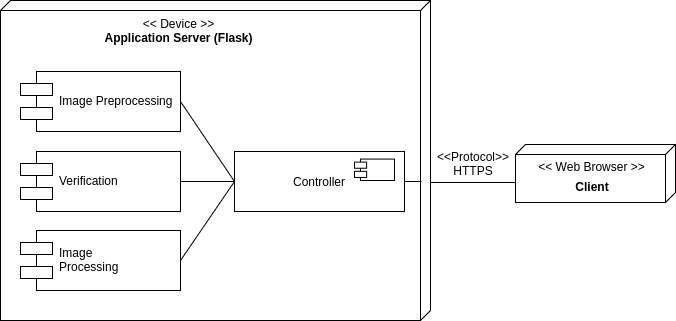
\includegraphics[scale=0.5]{img/Quant.png}
	    	\caption{Deployment Diagram of Hutts Verification}
	    \end{figure}
	    \pagebreak
	 
\section{Services}
This section outlines the design of each individual service and in terms of UML diagrams and how services are related to one another.

\subsection{Image Preprocessing Service}
The Image Preprocessing service is a crucial module of the system that requires a heavy emphasis. This service creates the image preprocessing pipeline for the application of all the necessary preprocessing techniques on incoming images to yield better results further down the system pipeline, specifically for further processing. This service is mostly used to prepare the image for OCR and facial recognition. 
\subsubsection{Class Diagram}
The class diagram of the Image Preprocessing module makes use of a well-known design pattern: 
\begin{itemize}
	\item \textbf{Builder:} Allows us to separate the representation of the pipeline from its construction. As a result, we can use the same construction process to create different pipelines, depending on the situation and type of ID document.
\end{itemize}
	\begin{figure}[H]
	    \centering
	    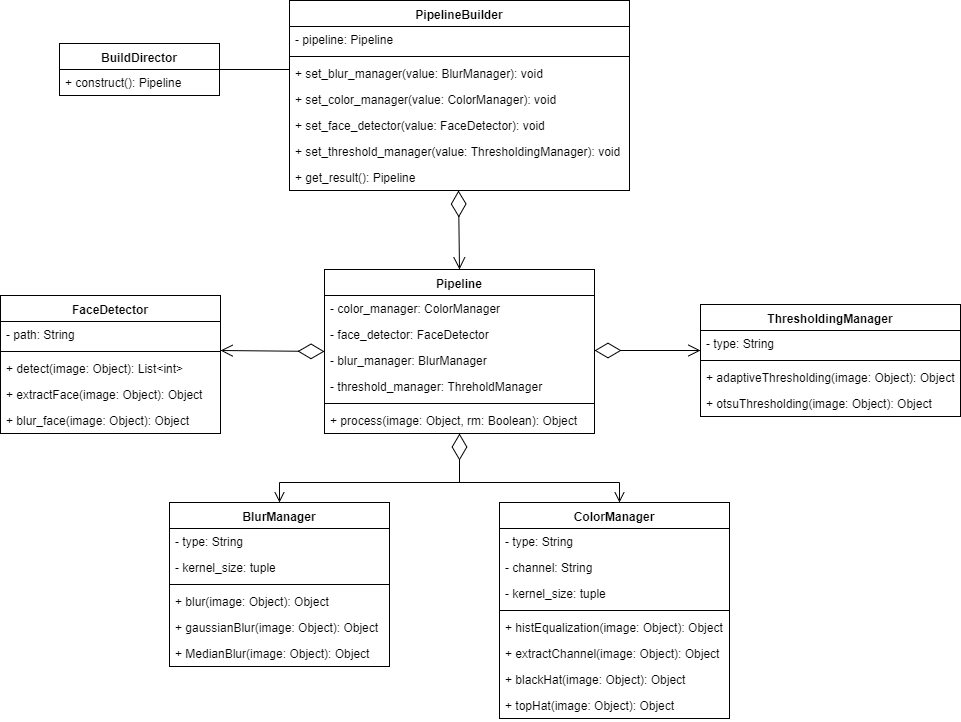
\includegraphics[scale=0.5]{img/imageProcessingClassDiagram.png}
	    \caption{Image Preprocessing Service}
	 \end{figure}
	 \pagebreak
\subsubsection{Activity Diagram}
    \begin{itemize}
        \item \textbf{Precondition:} A photo of an ID with a high DPI and reasonable, proportionate lighting should be
provided.
        \item \textbf{Postcondition:} The service returns a fully preprocessed image ready for extraction.
    \end{itemize}
	\begin{figure}[H]
	    \centering
	    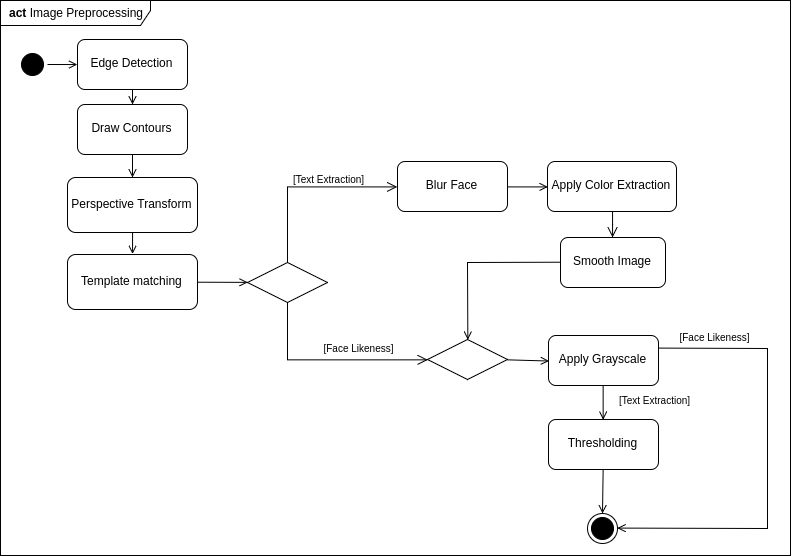
\includegraphics[scale=0.5]{img/activity_preprocessing.png}
	    \caption{Image Preprocessing Activity Diagram}
	 \end{figure}
	 \pagebreak

\subsection{Image Processing Service}
The Image Processing service is the core module of the system. This service creates the image processing pipeline by applying all the necessary computer vision and processing techniques. This service is mostly used to process the information contained within an incoming image into a workable format. 
\subsubsection{Class Diagram}
	\begin{figure}[H]
	    \centering
	    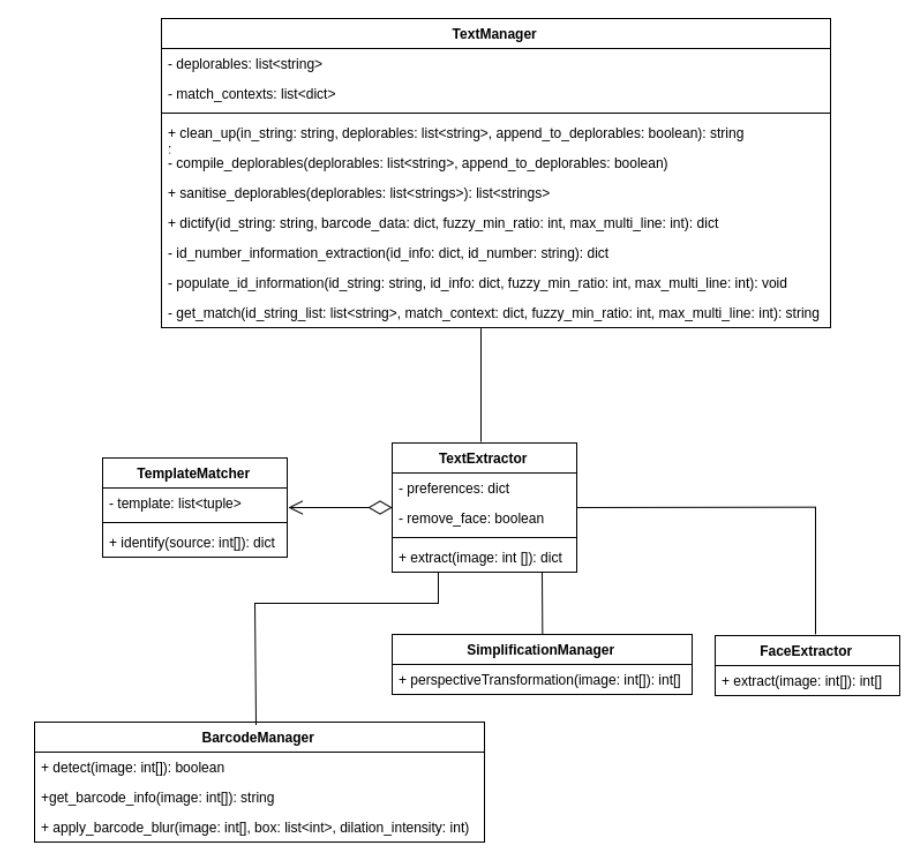
\includegraphics[scale=0.5]{img/extractClassDiagram.png}
	    \caption{Image Processing Service}
	 \end{figure}
	 \pagebreak
\subsubsection{Activity Diagram}
\begin{itemize}
        \item \textbf{Precondition:} A fully preprocessed image must be provided.
        \item \textbf{Postcondition:} The service returns the extracted text and face.
    \end{itemize}
	\begin{figure}[H]
	    \centering
	    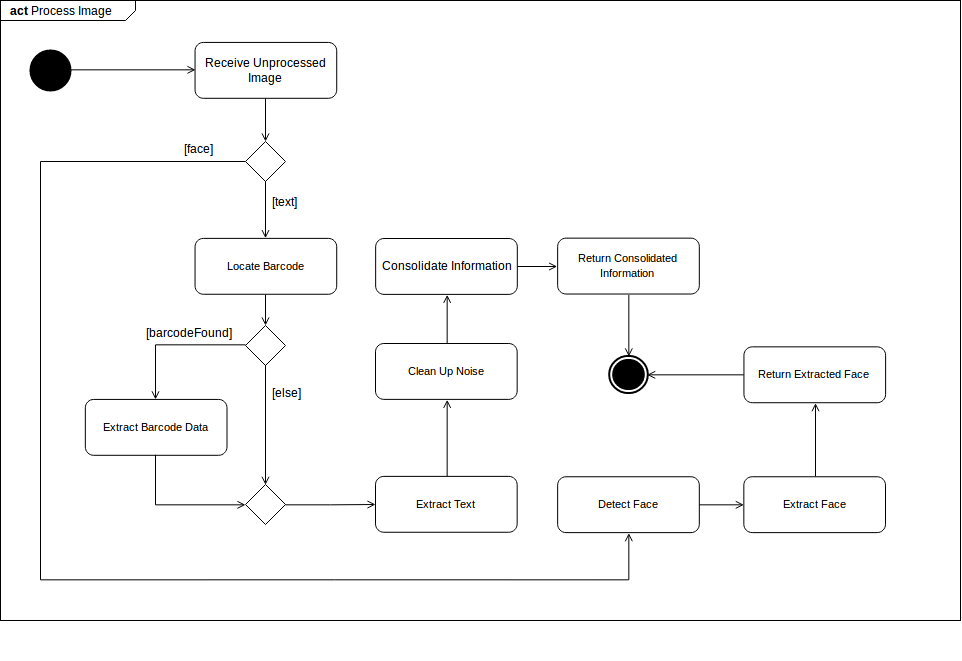
\includegraphics[scale=0.5]{img/process_activity.png}
	    \caption{Image Processing Activity Diagram}
	 \end{figure}
	 \pagebreak
\subsubsection{Sequence Diagram}
\begin{figure}[H]
	    \centering
	    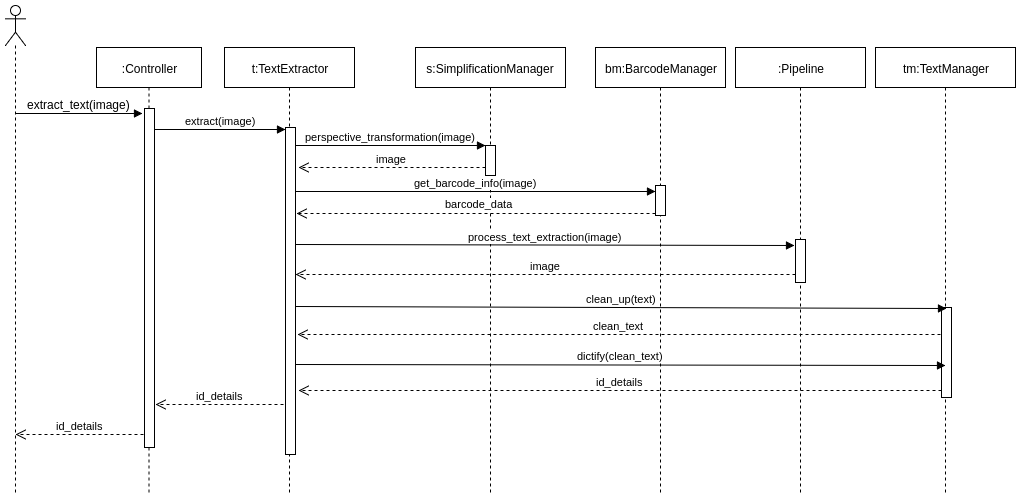
\includegraphics[scale=0.5]{img/extract_sequence.png}
	    \caption{Image Processing Sequence Diagram}
	 \end{figure}
	 \pagebreak
	 
\subsection{Verification Service}
The Verification service is the part of the system that is responsible for all the logic related to verifying a form of ID against given information. It performs the required checks and calculations to determine a likeness percentage that forms the ultimate verifier.
\subsubsection{Class Diagram}
	\begin{figure}[H]
	    \centering
	    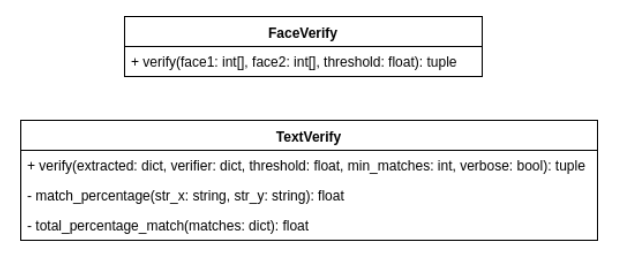
\includegraphics[scale=0.5]{img/VerifyClass.png}
	    \caption{Verification Service}
	 \end{figure}
	 \pagebreak
\subsubsection{Activity Diagram}
\begin{itemize}
        \item \textbf{Precondition:} A photo of an ID with a high DPI and reasonable, proportionate lighting should be
provided, as well as initial personal information and a photo of the individual's face.
        \item \textbf{Postcondition:} The service returns an overall percentage match for the data, as well as individual matches for text verification and face verification.
    \end{itemize}
	\begin{figure}[H]
	    \centering
	    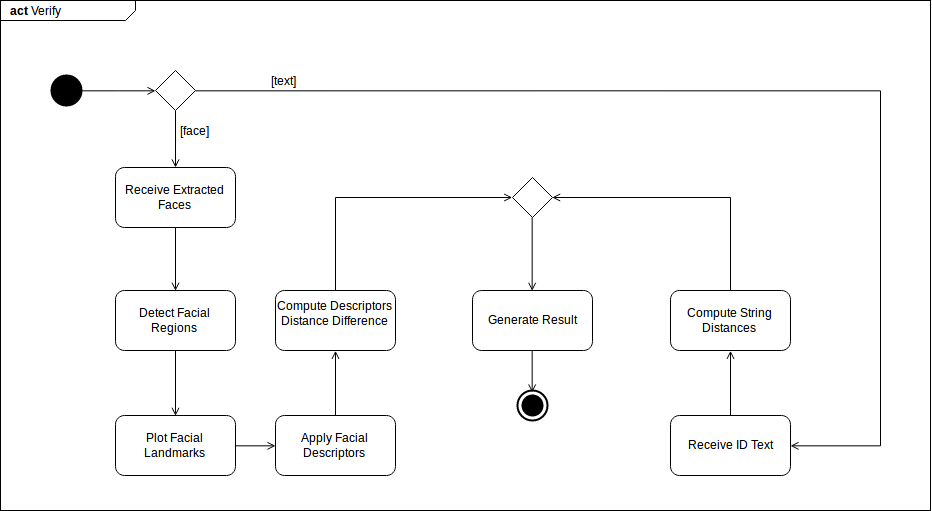
\includegraphics[scale=0.5]{img/verify_activity.png}
	    \caption{Verification Activity Diagram}
	 \end{figure}
	 \pagebreak
\section{High Level Diagrams}

\subsection{State Diagram}
\begin{figure}[h]
	\centering
	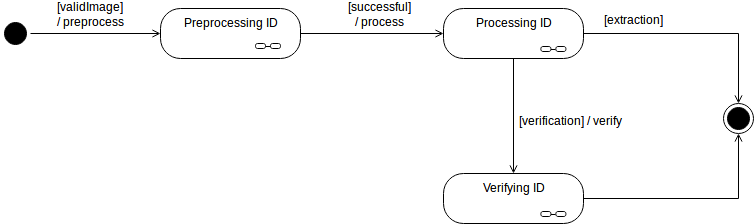
\includegraphics[scale=0.5]{img/StateModelHighLevel.png}
	\caption{High Level State Diagram}
\end{figure}

\subsection{Activty Diagrams}
\subsubsection{Verification}
	\begin{figure}[h]
		\centering
		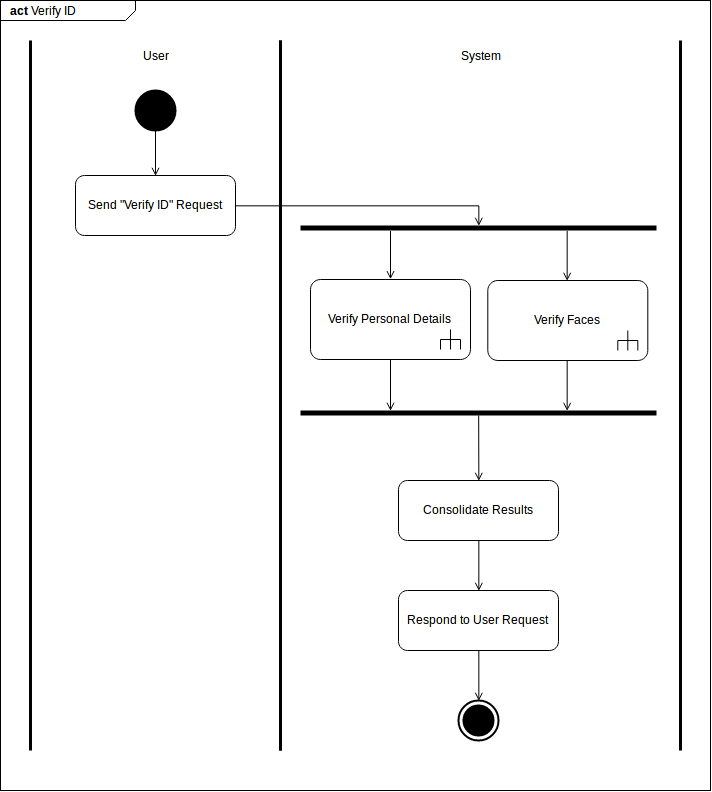
\includegraphics[scale=0.4]{img/verify_id_activity.png}
		\caption{Verify ID Activity Diagram}
	\end{figure}
\pagebreak
	\begin{figure}[h]
		\centering
		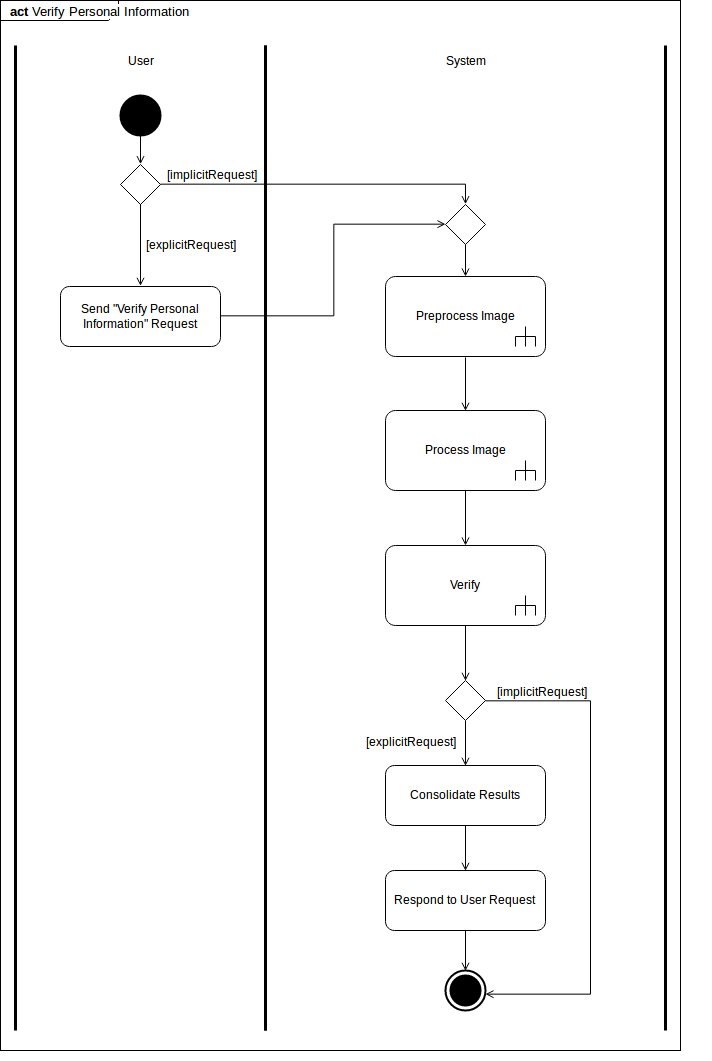
\includegraphics[scale=0.455]{img/verify_personal_info_activity.png}
		\caption{Verify Personal Information Activity Diagram}
	\end{figure}
\pagebreak
	\begin{figure}[!h]
		\centering
		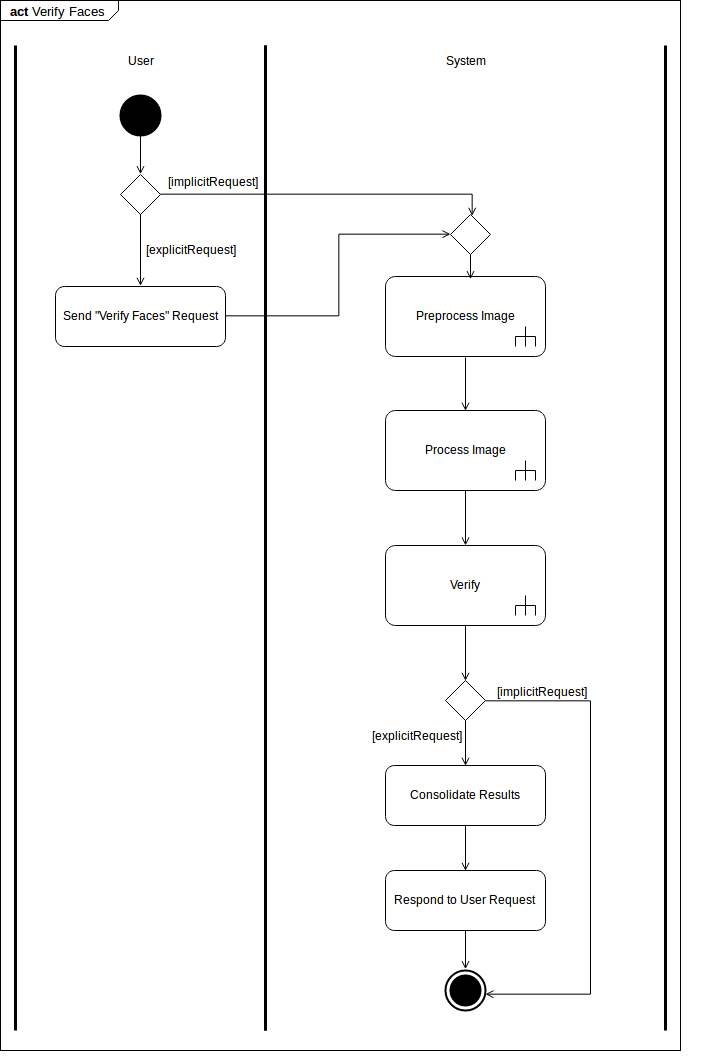
\includegraphics[scale=0.455]{img/verify_faces_activity.png}
		\caption{Verify Faces Activity Diagram}
	\end{figure}
\pagebreak
\subsubsection{Extraction}
	\begin{figure}[!h]
		\centering
		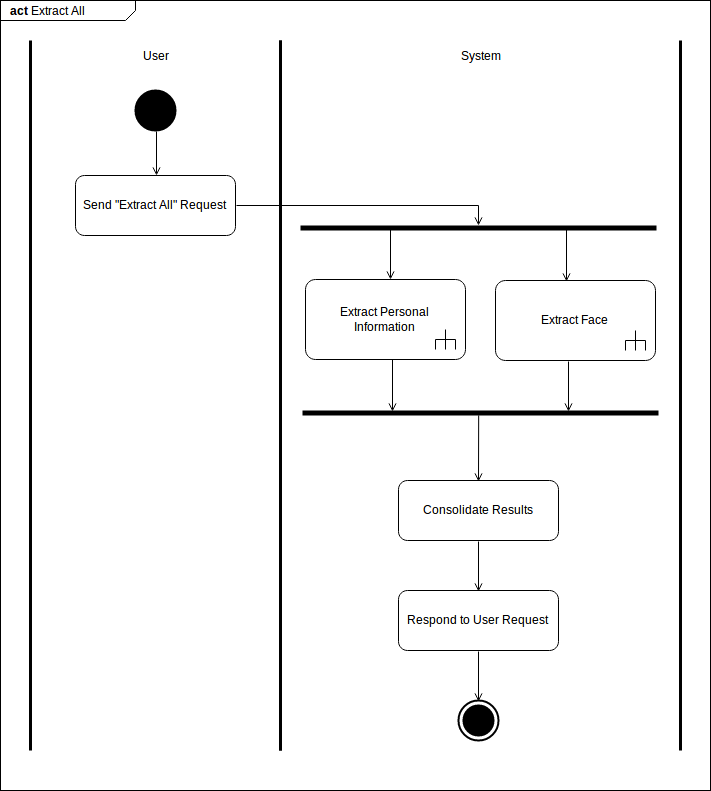
\includegraphics[scale=0.65]{img/extract_all_activity.png}
		\caption{Extract All Activity Diagram}
	\end{figure}
\pagebreak
	\begin{figure}[h]
		\centering
		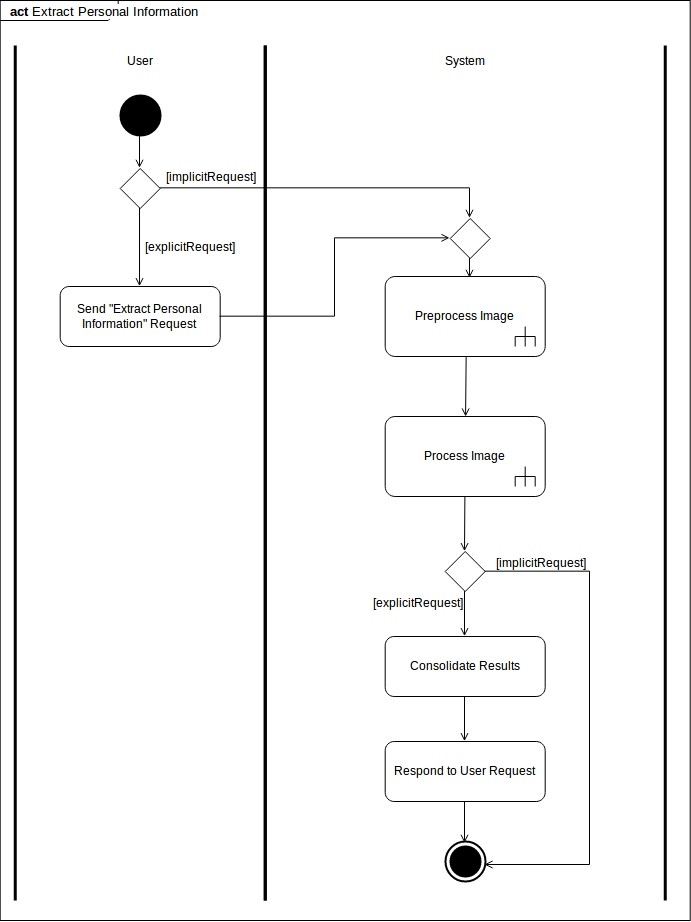
\includegraphics[scale=0.5]{img/extract_personal_info_activity.png}
		\caption{Extract Personal Information Activity Diagram}
	\end{figure}
\pagebreak
	\begin{figure}[h]
		\centering
		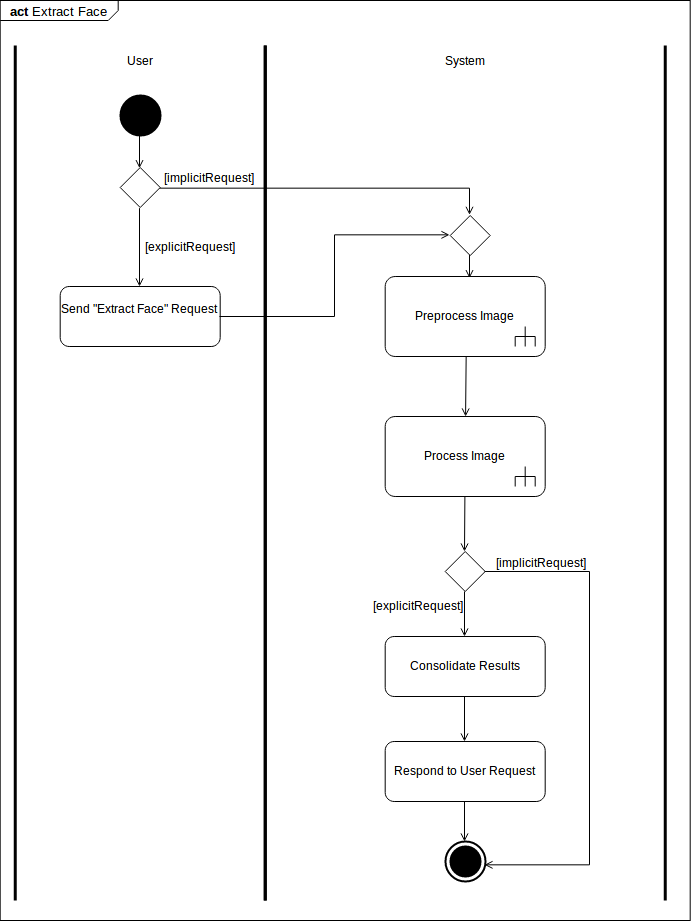
\includegraphics[scale=0.5]{img/extract_face_activity.png}
		\caption{Extract Face Activity Diagram}
	\end{figure}
\pagebreak
\end{document}
